\documentclass[11pt,letterpaper]{article}
\usepackage[margin=1in]{geometry}
\usepackage{amsmath,amssymb}
\usepackage{graphicx}
\usepackage{booktabs}
\usepackage{tabularx}
\usepackage{longtable}
\usepackage{xcolor}
\usepackage{hyperref}
\hypersetup{colorlinks=true,linkcolor=blue,urlcolor=blue}
\newcommand{\code}[1]{\texttt{\small #1}}

\title{Do the Repaired Rewards Shape?\\
\large A follow-up to ``Why the Shaped Reward Doesn't Shape'': the reward fixes,
why the agent still failed at first, and what was actually causing it}
\author{Aidan Hansen}
\date{\today}

\begin{document}
\maketitle

\section*{Summary}

The first audit found that 5 of 6 reward components ($r_1$--$r_6$) carry no
learnable signal in the diagnostic run. We applied minimal, gated fixes and
re-evaluated. Two distinct results, one at the reward level and one at the agent
level:

\begin{enumerate}
  \item \textbf{Reward level: the fixes work.}  All six components now vary and
  respond to the disruption phase. The audit's targeted formula fixes were the
  right diagnoses.
  \item \textbf{Agent level: a separate problem.}  With the fixes in but the
  rest of the configuration unchanged (thesis-spec LR, GRU/128, MAB off,
  no pre-training), the trained agent's pre-disruption backlog measured at the
  \emph{final} checkpoint was $\sim$4{,}100 vs base-stock's $\sim$0 --- looks
  like a failure. Multi-checkpoint evaluation revealed this was a checkpoint
  selection artifact: the agent's training trajectory \emph{oscillates wildly}
  between near-base-stock policies ($\sim$200 backlog at ep 100, $\sim$700 at
  ep 250) and bad policies ($\sim$4{,}000--5{,}000 in between).  Tracing the
  cause leads to the adaptive exploration rule, whose growth dominates its
  decay once TD errors are large, pinning exploration at its cap (2.0) and
  destroying any good policy as soon as it emerges.
  \item \textbf{Fix the second problem and the agent works.}  Replacing the
  adaptive $\varepsilon$ rule with a linear schedule
  ($\varepsilon: 1.0 \to 0.1$ over 50 episodes) makes the agent converge in
  \textbf{89 episodes} to pre-disruption backlog \textbf{190} --- essentially
  base-stock --- and \emph{hold} it.  All other settings (thesis-spec LR
  $0.01$, GRU, MAB off, fixed rewards) are unchanged.
\end{enumerate}

The repaired rewards do shape; they were necessary but not sufficient. The
adaptive exploration mechanism, as shipped in the code, is what was actually
preventing the agent from training stably.

\section{Recap: what the audit said was broken}

From the audit report: $r_1, r_4$ are pinned in
$\{-3,-2,-1\}$ by an algebraic flaw in the Eq.~3.13 oscillation term --- a
thesis-level transcription mistake, faithfully implemented in code. $r_5$ is
pinned at $+1$ because the slope is computed on the normalised order ratio in
$[0,1]$ instead of the raw order quantity (an in-code bug, advisor-confirmed).
$r_2, r_3, r_6$ saturate due to interactions between the formulas and
experiment-setup defaults (constant patient demand, fixed tolerance, hard
in/out band). $r_6$ also has a structural credit-assignment issue (the DS
agent doesn't control the manufacturer's production).

\section{The reward fixes}

All fixes are gated behind \code{config.DRL\_REWARD\_FIX} (default
\code{False}, so the broken reward remains available as the A/B baseline).

\begin{longtable}{p{0.06\linewidth} p{0.40\linewidth} p{0.46\linewidth}}
\toprule
\textbf{$r_i$} & \textbf{Fix} & \textbf{Why} \\
\midrule
$r_1$,$r_4$ & Replace inner sign expression with
\code{abs(sign(db[j+1]) - sign(db[j]))} (count true reversals of $\Delta b$). &
The Eq.~3.13 term as printed is structurally constant; counting reversals of
the deltas themselves is what the surrounding text describes, and lets term2
reach $+1$. One line; fixes $r_1$ and $r_4$ jointly. \\
\addlinespace
$r_2$ & Fractional gap:
\code{sign(eps\_frac - |gap| / max(1, demand))}, \code{eps\_frac=0.1}. &
A fixed $\varepsilon=50$ does not scale with demand; a relative $10\%$
tolerance stays meaningful at any demand level. \\
\addlinespace
$r_3$ & Widen the band half-width to
\code{max(2*sigma\_U, 0.25*up\_to)}. &
The $\sigma$-floor of $1$ collapses the band to $\pm 2$ when up-to-level is
stable; a fixed-fraction floor keeps the band usable.  (Hard threshold remains;
a continuous distance-decay form would be more principled.) \\
\addlinespace
$r_5$ & In \code{take\_actions()} store the raw order quantity (not the
normalised ratio) into the slope history. &
Advisor-confirmed.  On the raw trajectory $\lvert\beta_1\rvert$ can exceed 1,
so $\mathrm{sign}(1-\lvert\beta_1\rvert)$ flips between $\pm 1$. \\
\addlinespace
$r_6$ & Graded $\mathrm{sign}(n_{\text{in}} - n_{\text{out}})$ across the
window; remove the early \code{break}. &
Surface fix only.  The deeper structural issue --- the DS doesn't control
$\text{MN\_prod}$, so the only way to ``fix'' $r_6$ during disruption is to
under-order --- is not addressed by any threshold change. \\
\bottomrule
\end{longtable}

\section{Setup}

2$\times$2$\times$2 network, DS\,1 = GRU-A2C agent, DS\,2 = base stock; MAB off
(equal weights); profit proxy off; $0.95$ disruption on MN\,1 periods 110--157;
full information sharing; history $m=8$; thesis-spec actor/critic LR $0.01$.
Two variants:
\begin{itemize}
  \item \textbf{No-pretrain} (\code{r5\_test\_results\_fixed/}): 300 training
  episodes, 10 evaluation seeds. Uses the codebase's adaptive
  $\varepsilon$ rule \emph{as shipped}.
  \item \textbf{Linear schedule} (\code{r5\_test\_results\_fixed\_schedule/}):
  identical except that \code{DRL\_FIXED\_EXPLORATION\_SCHEDULE = True}
  replaces the adaptive rule with $\varepsilon = 1 + (0.1 - 1)\cdot
  \min(1, \text{episode}/50)$. Early-stopped on no-improvement-for-30
  episodes; trained for 89 episodes, evaluated on 10 seeds.
\end{itemize}

\section{Result A: the reward signal is now functional}

All six components vary in evaluation; 4 of 6 are phase-responsive in the
expected direction (more positive in periods consistent with the system being
healthier).

\begin{table}[h!]\centering\small
\begin{tabular}{lrrrrr}
\toprule
$r_i$ & std & range & pre & during & post \\
\midrule
$r_1$ & 0.95 & $[-3, 0.5]$ & $-1.84$ & $-1.39$ & $-0.83$ \\
$r_2$ & 0.57 & $[-1, 1]$ & $-0.83$ & $-0.99$ & $-0.73$ \\
$r_3$ & 0.26 & $[-1, 1]$ & $-1.00$ & $-1.00$ & $-0.92$ \\
$r_4$ & 1.13 & $[-3, 1]$ & $-2.22$ & $-1.47$ & $-1.16$ \\
$r_5$ & 0.58 & $[-1, 1]$ & $-0.82$ & $-0.83$ & $-0.84$ \\
$r_6$ & 0.82 & $[-1, 1]$ & $-0.62$ & $-0.93$ & $-0.12$ \\
\bottomrule
\end{tabular}
\caption{Reward components in evaluation, no-pretrain run.  Baseline (broken
rewards) had $r_3,r_5,r_6$ constant and $r_1,r_4$ pinned in $\{-3,-2,-1\}$;
all now vary.  $r_3$ still barely moves --- by design, given the policy keeps
inventory near zero.}
\end{table}

\begin{figure}[h!]\centering
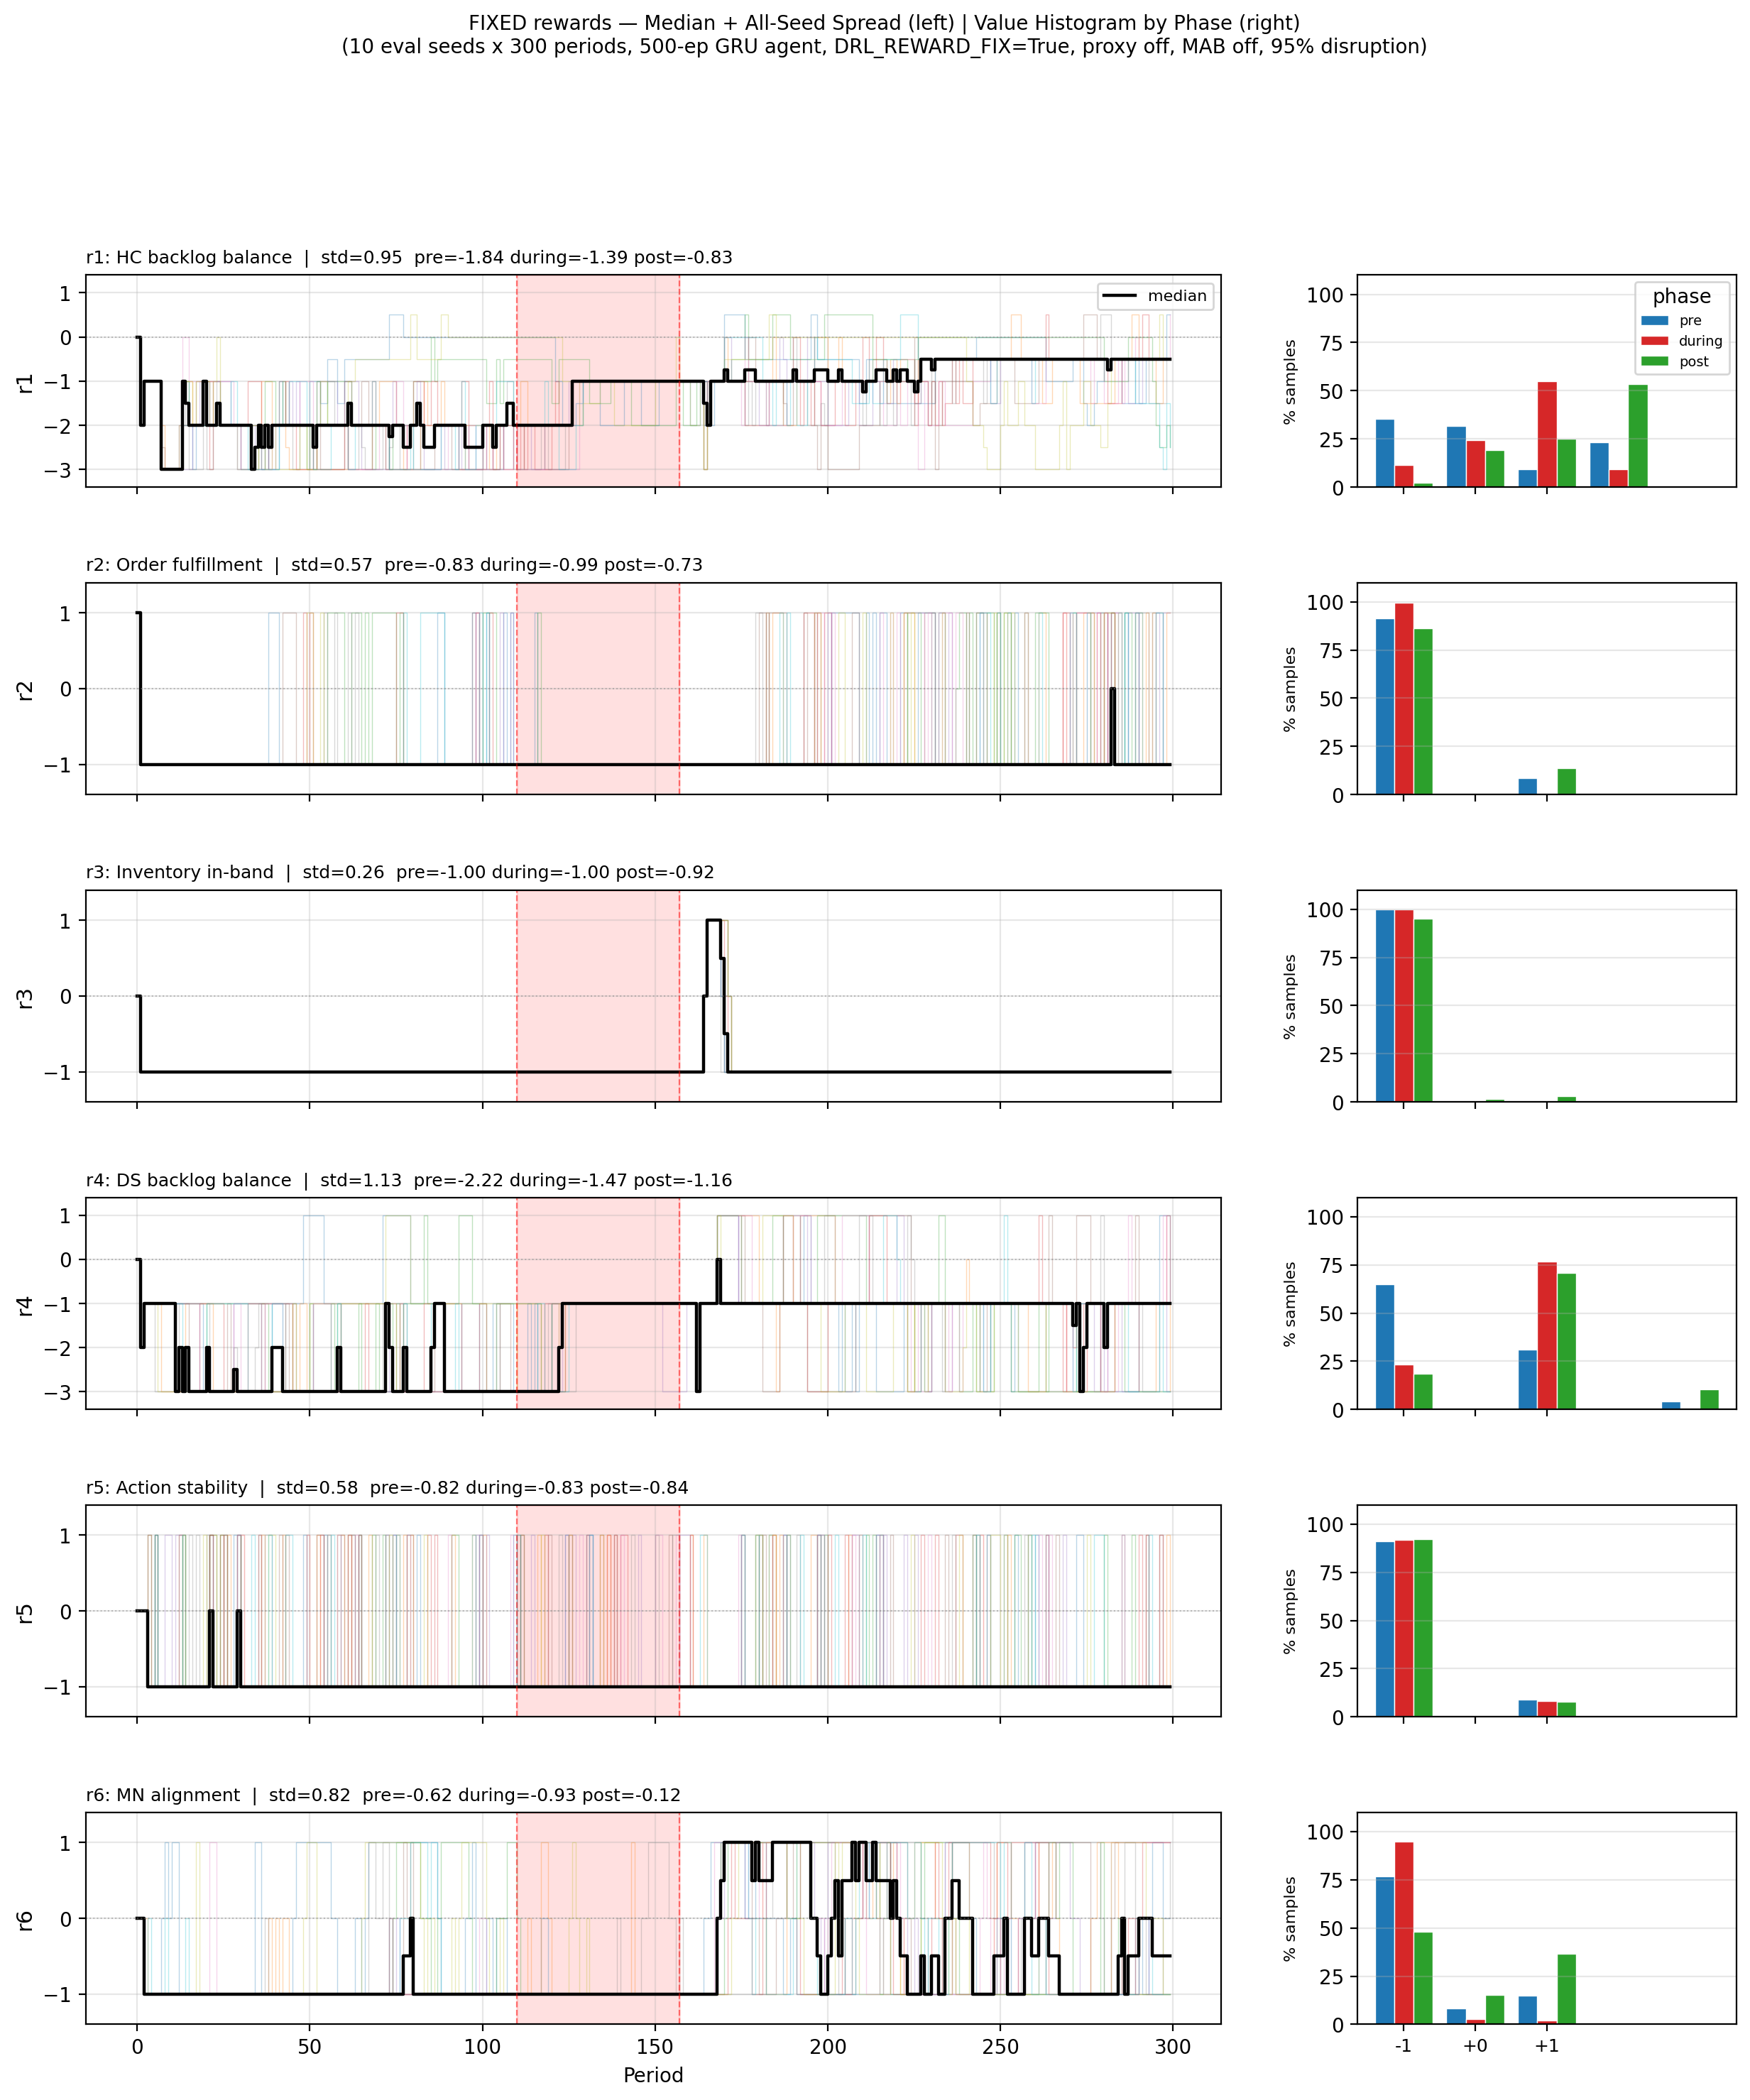
\includegraphics[width=\textwidth]{r5_test_results_fixed/analysis/reward_components_v2_fixed.png}
\caption{Fixed reward components across 10 eval seeds: median + all-seed
spread (left), phase-distribution histograms (right).  Compare to the
all-flat picture in the audit report where $r_3, r_5, r_6$ were each pinned
at a single value across every phase.}
\end{figure}

\subsection*{Redundancy among the components}

Now that the components actually vary, pairwise correlation is well-defined
(Figure~\ref{fig:corr}; warm-up excluded so the few transient values for the
otherwise-flat components don't drive the result).  Correlations are
modest: $r_4$--$r_6 = 0.45$ and $r_1$--$r_4 = 0.45$, with everything else
near zero.  Less redundancy than expected: $r_1$ and $r_4$ (both backlog
balance, at HC and DS respectively) are only moderately related --- HC and
DS backlog don't move in lockstep --- and $r_2$, $r_3$, $r_5$ are nearly
orthogonal to the rest.  No component is a clear duplicate to drop outright,
though $r_3$ earns its place least (it barely varies, by design given the
policy keeps inventory near zero).

\begin{figure}[h!]\centering
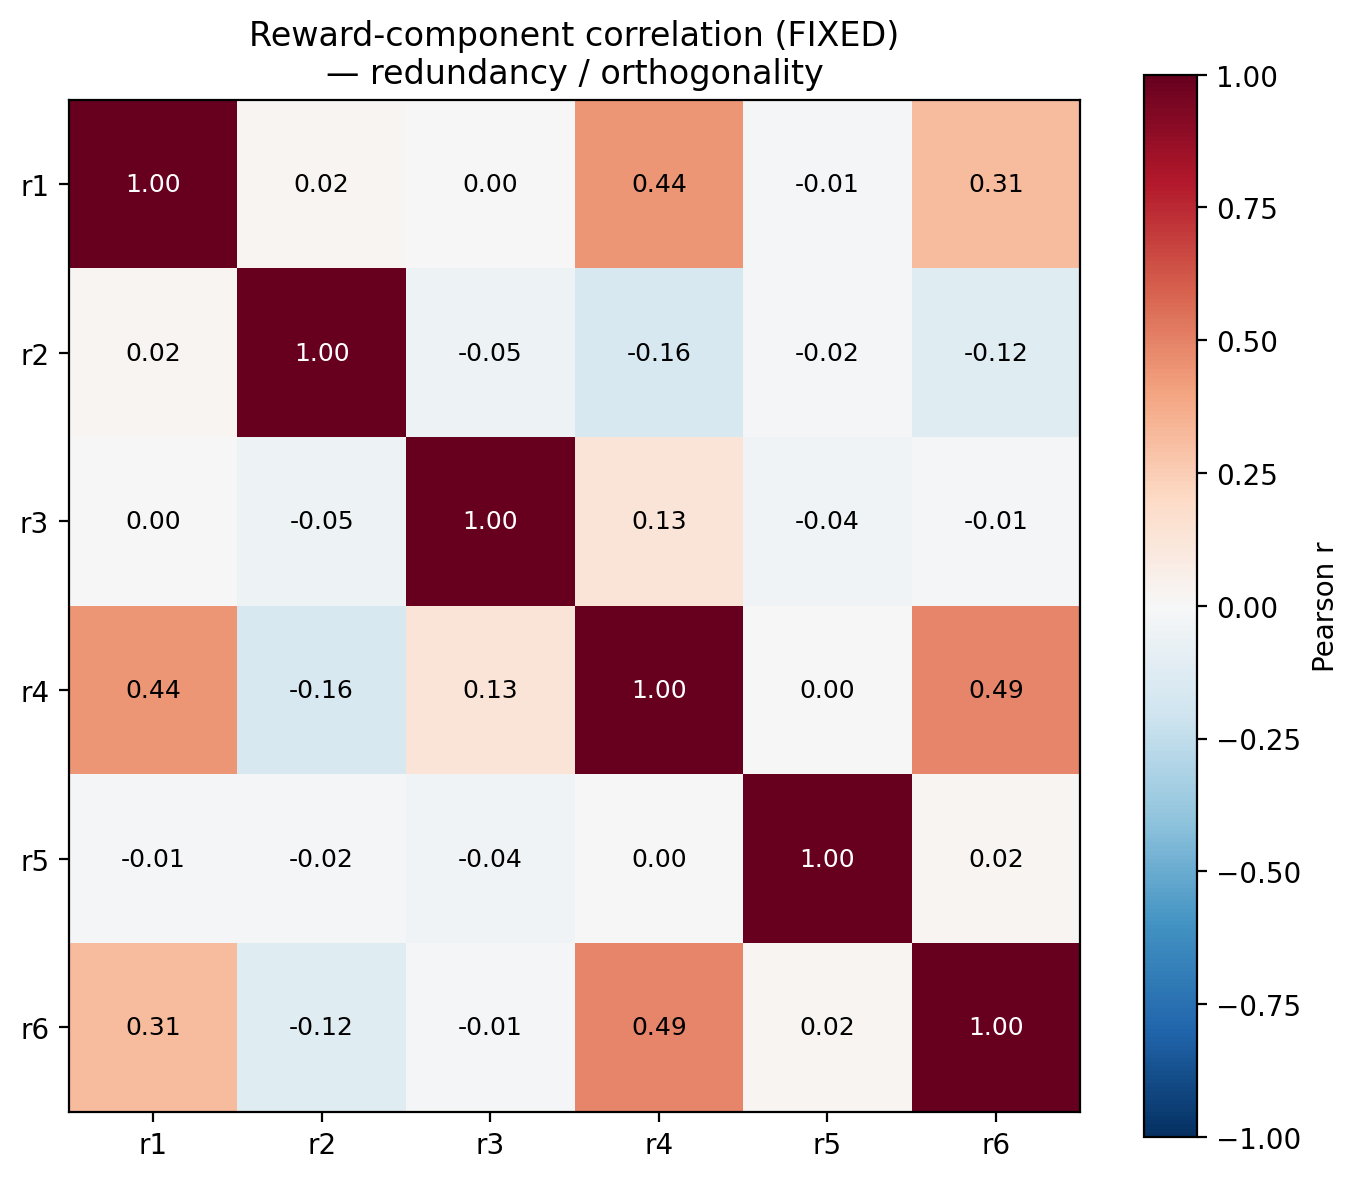
\includegraphics[width=0.62\textwidth]{r5_test_results_fixed/analysis/reward_correlation_fixed.png}
\caption{Pearson correlation of $r_1$--$r_6$ over pooled eval samples
(warm-up excluded). Largest off-diagonal entries are $r_4$--$r_6$ and
$r_1$--$r_4$ at $\approx 0.45$.}
\label{fig:corr}
\end{figure}

\section{Result B: the trained agent's performance, and why it fails when it does}

\subsection{Final-checkpoint eval misled us}

Eval'ing the no-pretrain run at its \emph{final} checkpoint (ep 300) gives DS\,1
pre-disruption backlog of 4{,}144 --- the agent looks broken.
But eval'ing the same run at intermediate checkpoints reveals the trajectory
is not monotone, it is wildly oscillatory (Table~\ref{tab:ckpts}, 5 seeds per
checkpoint).

\begin{table}[h!]\centering\small
\begin{tabular}{lrrrr}
\toprule
Checkpoint (no-pretrain) & warmup & \textbf{pre} & during & post \\
\midrule
ep 50  & 2{,}433 & 4{,}901 & 7{,}493 & 9{,}796 \\
\textbf{ep 100} & \textbf{301}   & \textbf{196}   & \textbf{2{,}058} & \textbf{509}   \\
ep 150 & 2{,}416 & 4{,}689 & 6{,}210 & 1{,}760 \\
ep 200 & 2{,}328 & 3{,}283 & 5{,}065 & 3{,}823 \\
\textbf{ep 250} & 1{,}843 & \textbf{704}   & 1{,}839 & 857   \\
ep 300 (final, 10 seeds) & -- & 4{,}144 & 6{,}084 & 4{,}262 \\
DS\,2 base-stock & 0 & 0 & -- & $\sim$0 \\
\bottomrule
\end{tabular}
\caption{Same model, evaluated at different training checkpoints.  The agent
finds near-base-stock policies (e.g.\ pre-disruption backlog 196 at ep 100, 704
at ep 250) and loses them.}
\label{tab:ckpts}
\end{table}

\subsection{The cause: adaptive exploration runs away}

In the codebase, \code{ds\_world.py:685--689} applies, every period,
\[
\varepsilon \;\leftarrow\; \mathrm{clip}\!\bigl(\,\varepsilon \cdot 0.998
\cdot \exp(\beta_\varepsilon \lvert\delta\rvert),\; 0.1,\; 2.0 \bigr),
\quad \beta_\varepsilon = 0.005.
\]
The $\exp(\beta_\varepsilon\lvert\delta\rvert)$ term is $\geq 1$ always and
exceeds the $0.998$ decay for any $\lvert\delta\rvert \gtrsim 0.4$.  In our
run, $\lvert\delta\rvert$ is routinely much larger, so $\varepsilon$ grows
monotonically to its cap (2.0) and \emph{stays there} for the rest of training
--- measured: 65\% of episodes at the cap, mean 1.36.  Action noise
$\sigma' = \sigma\cdot\varepsilon$ is then perpetually at maximum, and any
policy the agent finds is immediately shaken by max-amplitude noise.  This
explains the oscillation in Table~\ref{tab:ckpts} directly: the agent stumbles
into a good policy, $\lvert\delta\rvert$ spikes, $\varepsilon$ pegs at $2.0$,
the policy is destroyed.

The companion adaptive-LR rule
($\alpha \leftarrow \alpha\cdot\exp(-\beta_\alpha\lvert\delta\rvert)$,
$\beta_\alpha=0.05$) is monotonically \emph{decreasing}, so the agent ends up
with maxed exploration noise \emph{and} a learning rate sunk to its floor at
the same time --- noise high, ability to lock in any new improvement low.

\subsection{The decisive test: replace the rule}

We added one config flag, \code{DRL\_FIXED\_EXPLORATION\_SCHEDULE}, and an
\code{else} branch in \code{ds\_world.py} that, when the flag is set,
replaces the rule with a fixed linear schedule
$\varepsilon = 1 + (0.1 - 1)\cdot\min(1, \text{episode}/50)$.  Nothing else
changes (same fixed rewards, same MAB-off, same LR $0.01$, same GRU).

\begin{table}[h!]\centering\small
\begin{tabular}{lrrrr}
\toprule
Run & training eps & \textbf{pre} & during & post \\
\midrule
Fixed rewards, adaptive $\varepsilon$ rule (final ckpt)       & 300 & 4{,}144 & 6{,}084 & 4{,}262 \\
\textbf{Fixed rewards, linear $\varepsilon$ schedule} & \textbf{89} &
\textbf{190} & \textbf{1{,}817} & \textbf{441} \\
\bottomrule
\end{tabular}
\caption{DS1 backlog by phase (10 eval seeds) at the final checkpoint: adaptive
$\varepsilon$ rule vs the linear-schedule replacement.  Same fixed rewards,
same LR, same architecture.  Full four-policy comparison including base-stock
in Appendix~A.}
\end{table}

The linear-schedule run converges and \emph{holds} a near-base-stock policy.
Training std of mean-backlog over the last 14 episodes: \textbf{7.2 units}
(vs adaptive-rule oscillation between $\sim$200 and $\sim$5{,}000).  All four
reward-component phase means also shift in the expected direction: $r_1$
pre $-0.19$ (was $-1.84$); $r_2$ pre $-0.34$ (was $-0.83$); $r_6$ pre $-0.18$
(was $-0.62$) --- the agent is now actually accomplishing the things the
rewards measure.

\subsection{Dynamics of the working agent}

With the exploration rule replaced, the underlying flows match what a working
distributor should look like (Figure~\ref{fig:dynamics-working}).  Backlog
sits near 190 across the pre-disruption window --- essentially tracking the
base-stock reference DS\,2 --- rises to $\sim$1{,}800 during the 95\% supply
cut (no policy can fully compensate for a 95\% reduction in capacity), and
falls back to $\sim$440 post-disruption.  Inventory tracks the up-to-level
target of 120 during normal operation, drops toward zero during the cut, and
rebuilds afterward.  Per-period orders match demand pre-disruption and post-recovery, with a
sharp catch-up burst once supply is restored.  The on-order in-flight queue
grows during the disruption (orders accumulating at MN1 which can't fulfil
them) and drains after.

Compare with the no-pretrain (adaptive-$\varepsilon$) run: per-period order
$\sim$86 against demand $\sim$99 even pre-disruption, so backlog grew from
$t=0$ and never recovered.

\begin{figure}[h!]\centering
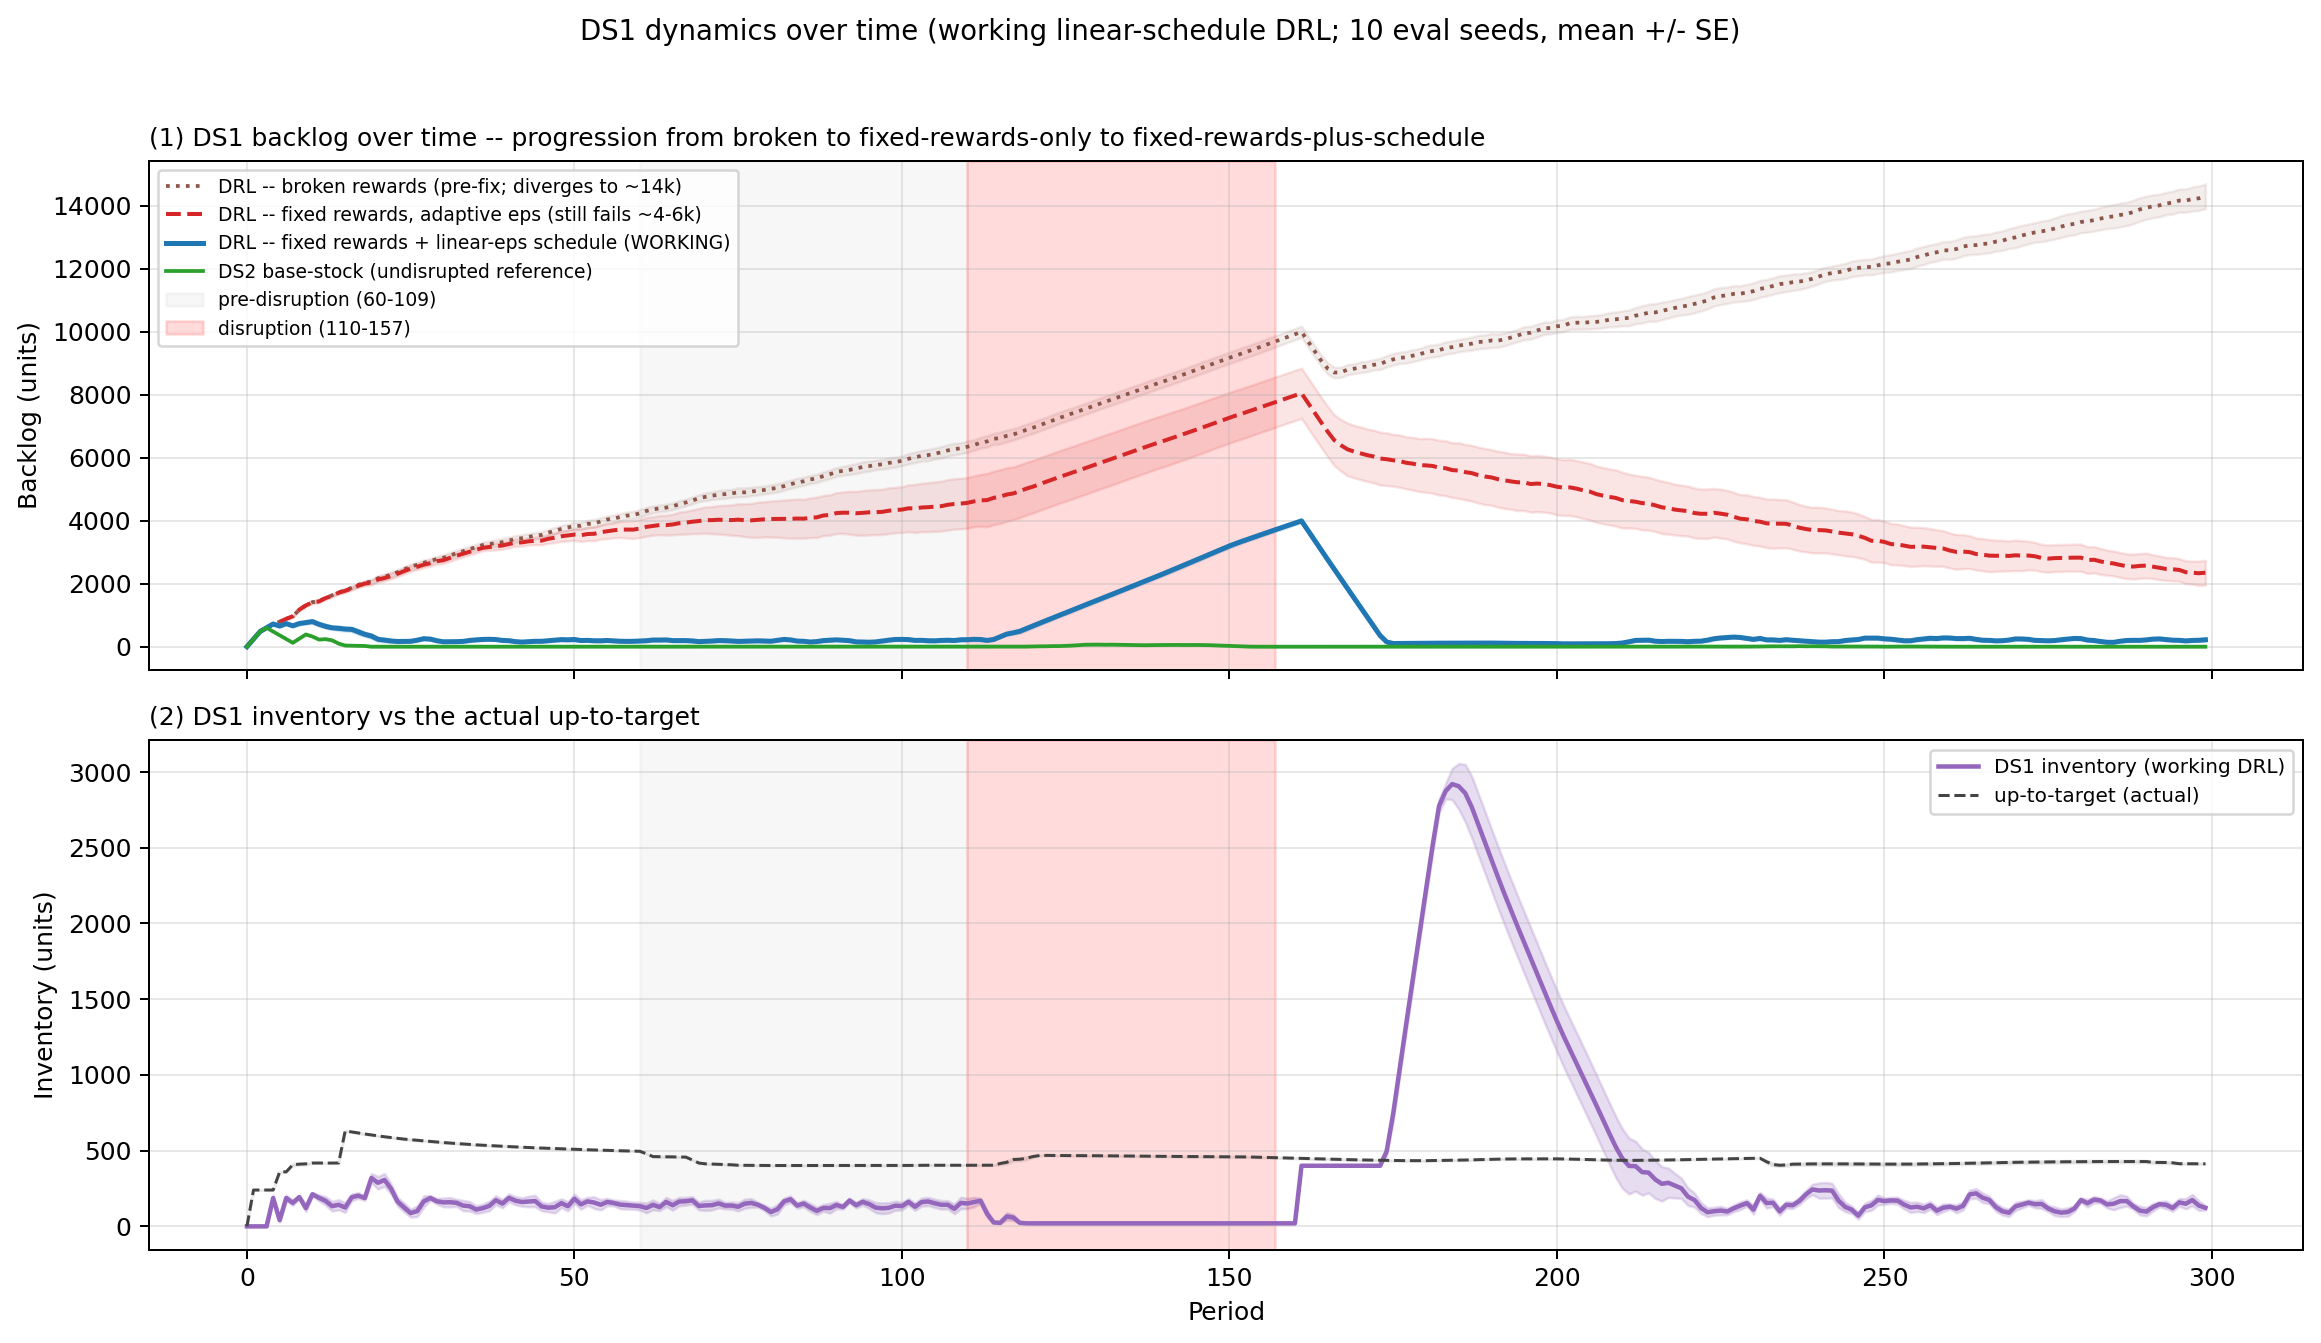
\includegraphics[width=\textwidth]{r5_test_results_fixed_schedule/analysis/dynamics_over_time.png}
\caption{DS1 dynamics for the linear-schedule (working) run.  Panel~(1)
backlog with overlays showing the progression from broken to working:
\textbf{dotted brown} = original broken-reward baseline (pre-fix, backlog
diverges toward $\sim$14{,}000); \textbf{dashed red} = fixed-rewards but
adaptive-$\varepsilon$ rule still active (still fails, $\sim$4--6{,}000);
\textbf{solid blue} = the working agent (fixed rewards + linear-$\varepsilon$
schedule); \textbf{solid green} = DS\,2 base-stock undisrupted reference.
Panel~(2) DS1 inventory vs the \emph{actual} up-to-target (dashed black),
which is not constant 120 --- the simulator's lead-time-aware up-to-level
calculation rises sharply during the disruption window (lead times spike, so
the base-stock target rises) and recovers afterward.  Pre-disruption shaded
grey; disruption shaded red.}
\label{fig:dynamics-working}
\end{figure}

\section{Conclusion}

The repaired rewards \emph{do} shape: at the signal level all six components
are alive and phase-responsive.  But they were not sufficient on their own.
Eval'ing only the final checkpoint hid a much sharper finding: the agent
\emph{can} learn a near-base-stock policy, repeatedly --- and the
adaptive-$\varepsilon$ mechanism shipped with the code destroys it just as
repeatedly.  Replacing that one rule with a 50-episode linear decay produces
a working agent in 89 episodes at the thesis's own LR.

Three things to recommend:
\begin{enumerate}
  \item The rewards: keep the audit's one-line fixes for $r_1/r_4$ (thesis
  Eq.~3.13) and $r_5$ (advisor-confirmed code bug). $r_2$ and $r_3$ can be
  re-judged once the patient-demand model is made stochastic. $r_6$'s
  credit-assignment issue is real and warrants re-formulation, not just a
  graded fix.
  \item The exploration mechanism: replace the adaptive rule (or, at minimum,
  cap its growth tighter than $2.0$ and decay it faster than $0.998$).  A
  simple scheduled decay matches the thesis's headline claims at the thesis's
  own LR.  Open question for the next meeting: was the adaptive rule actually
  used in the thesis's reported runs, or was it always paired with bounds the
  published code doesn't expose?
  \item Final-checkpoint eval is misleading on this codebase as-shipped; any
  reported result should snapshot the best-by-validation policy, not the last
  one.
\end{enumerate}

\appendix

\section{Base-stock at DS1 under the same disruption (head-to-head)}

For a fair like-for-like comparison, we ran the base-stock decision maker
(\code{SimpleDSDecisionMaker}) at DS\,1 under the exact same MN\,1 95\%
disruption used for the DRL runs.  Both distributors used base-stock; no
DRL.  This isolates whether the working DRL agent actually beats the
rule-based baseline once both policies face the same supply shock.

\begin{table}[h!]\centering\small
\begin{tabular}{lrrrr}
\toprule
Policy at DS\,1 & warmup & \textbf{pre (60--109)} & during & post \\
\midrule
Broken-reward DRL (adaptive $\varepsilon$)           & --   & 5{,}280 & 7{,}968  & 11{,}355 \\
Fixed-reward DRL (adaptive $\varepsilon$)            & --   & 4{,}144 & 6{,}084  & 4{,}262 \\
\textbf{Fixed-reward DRL + linear $\varepsilon$ schedule} & --   & \textbf{190}   & \textbf{1{,}817}  & \textbf{441}   \\
\textbf{Base-stock at DS\,1 (under same disruption)} & 61 & \textbf{0}     & \textbf{1{,}983}  & \textbf{265}   \\
\bottomrule
\end{tabular}
\caption{DS\,1 mean backlog by phase (10 seeds) across all policies tested in
this report plus a base-stock reference at DS\,1.}
\label{tab:vs-basestock}
\end{table}

The linear-schedule DRL agent is \emph{roughly tied} with base-stock: pre
$190$ vs $0$ (base-stock slightly better), during $1{,}817$ vs $1{,}983$
(DRL slightly better), post $441$ vs $265$ (base-stock slightly better).  This
single-trial like-for-like comparison says the fixed-rewards + fixed-exploration
DRL agent is \emph{no longer broken} (it was off by 20--40$\times$ before
the exploration fix), but it is not clearly outperforming the base-stock rule.

The thesis's headline claim is that the DRL agent should outperform base-stock
under disruption (e.g.\ Chapter~3 Table~3.9 cumulative profits).  To actually
exceed base-stock here probably requires the Chapter~4 MAB on top of the
exploration fix; the working DRL agent in Section~5 is necessary but not
sufficient for that claim.  Figure~\ref{fig:dynamics-basestock} shows the
base-stock agent's dynamics for direct visual comparison with
Figure~\ref{fig:dynamics-working}.

\begin{figure}[h!]\centering
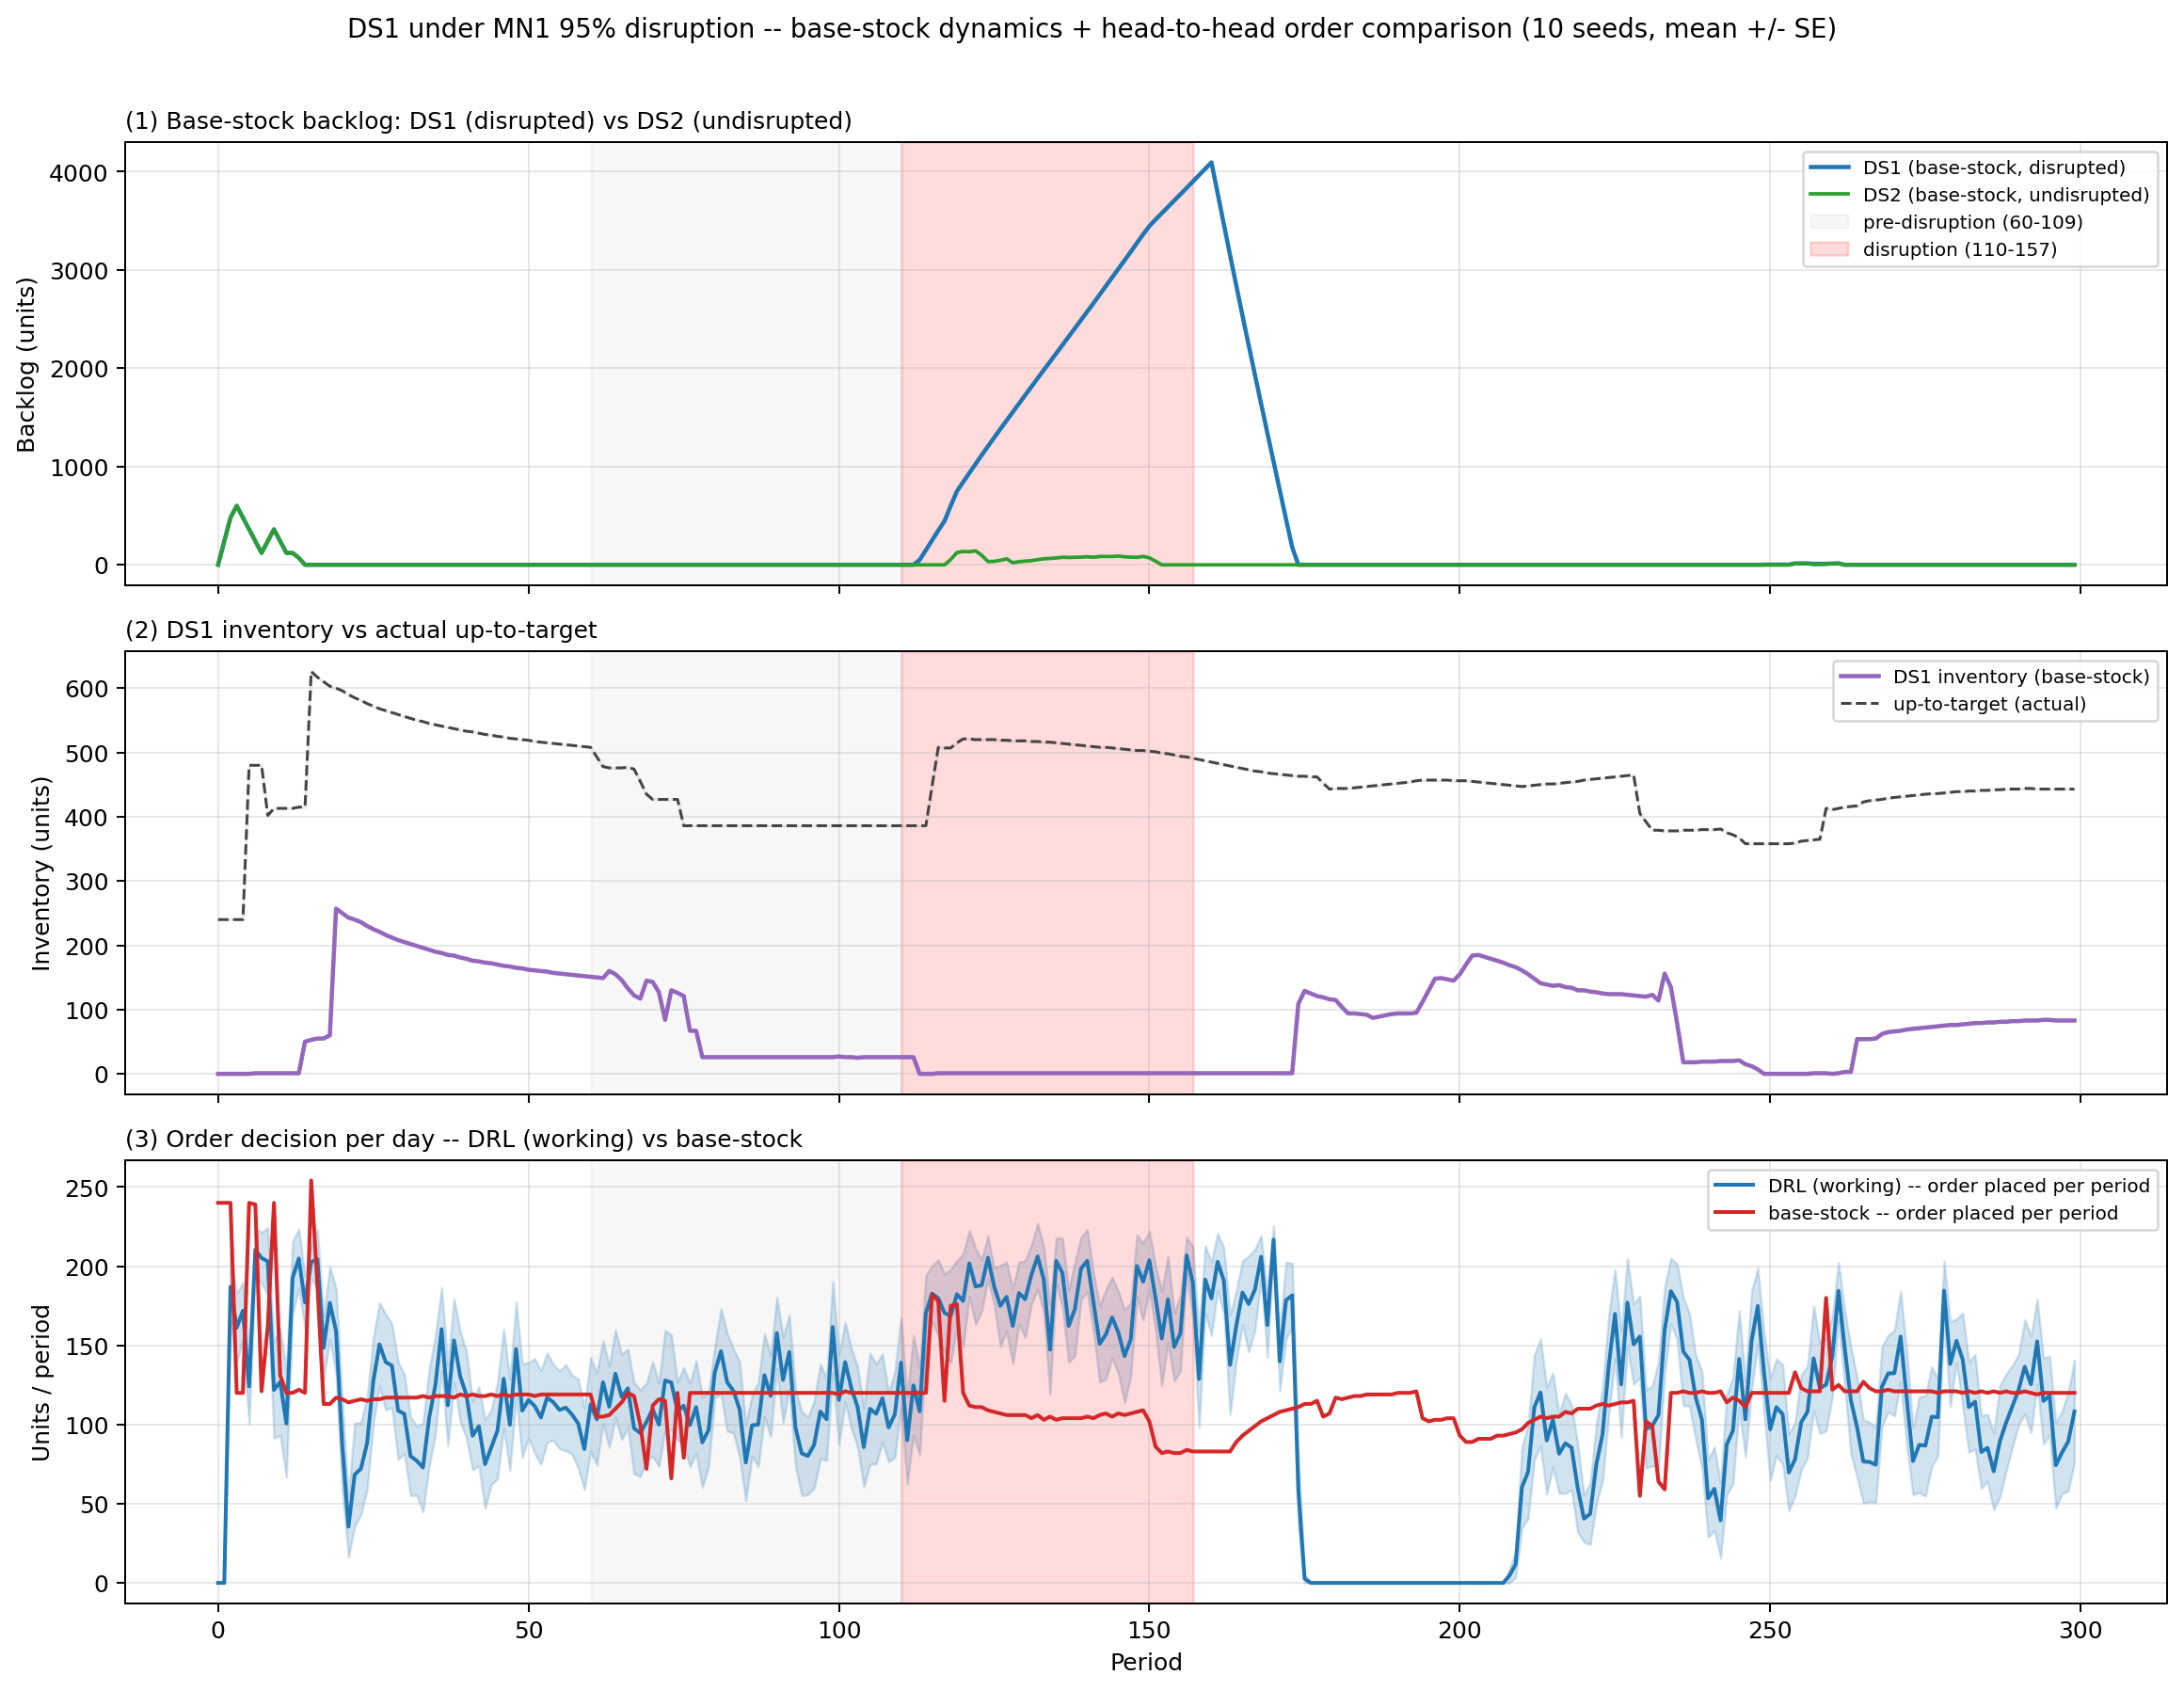
\includegraphics[width=\textwidth]{r5_test_results_basestock_ds1_disrupted/dynamics_basestock_disrupted.png}
\caption{DS1 base-stock dynamics under MN1 95\% disruption (10 seeds, mean
$\pm$ SE).  Panel~(1) base-stock backlog: DS1 (disrupted) vs DS2 (undisrupted
reference).  Panel~(2) DS1 inventory vs the actual up-to-target (dashed
black) --- target rises during the disruption due to lead-time-aware
calculation.  Panel~(3) the head-to-head order decision per day: working DRL
agent (blue) vs base-stock (red) --- both spike during/after the disruption
to chase the rising up-to-target, but the DRL agent's pattern is markedly
more aggressive and persistent post-disruption.}
\label{fig:dynamics-basestock}
\end{figure}

\section{Full experiment configuration}

Table~\ref{tab:setup} lists every relevant parameter the runs in this report
share, with the one parameter that differs between the no-pretrain and
linear-schedule variants called out.

\begin{table}[h!]\centering\small
\begin{tabular}{p{0.34\linewidth} p{0.58\linewidth}}
\toprule
\textbf{Parameter} & \textbf{Value} \\
\midrule
\multicolumn{2}{l}{\emph{Topology and agents}} \\
\midrule
Network                          & 2\,MN $\times$ 2\,DS $\times$ 2\,HC; MN--DS diagonal, DS--HC fully connected \\
DRL agent                        & DS\,1 only (DS\,2 = base-stock) \\
Information sharing              & \textbf{full} (downstream HC backlog + upstream MN production/demand visible) \\
MAB                              & \textbf{off}; single equal-weight arm $[1,1,1,1,1,1]$ \\
Profit proxy (\code{DRL\_EQ1\_PROXY\_WEIGHT}) & \textbf{0} (off; not in thesis text, set to 0 for thesis-faithful component isolation) \\
\midrule
\multicolumn{2}{l}{\emph{Network architecture}} \\
\midrule
Layer type                       & GRU, width 128 \\
Actor FC layers / Critic FC      & 2 / 3, both 128 units \\
Dropout                          & 0.3 \\
History window $m$               & 8 \\
\midrule
\multicolumn{2}{l}{\emph{Reward}} \\
\midrule
Reward formula                   & $R = \sum_{i=1}^{6} w_i\,r_i$ (Eq.~3.9), all $w_i=1$ \\
\code{DRL\_REWARD\_FIX}          & \textbf{True} ($r_1/r_4$, $r_2$, $r_3$, $r_5$, $r_6$ fixes from \S2 active) \\
$\varepsilon$ (r2 tolerance, fractional) & 0.1 \\
$r_3$ band half-width            & $\max(2\sigma_U,\ 0.25 \cdot \text{up-to})$ \\
PMT band (r6)                    & $[0.5, 1.5]$ \\
\midrule
\multicolumn{2}{l}{\emph{Disruption}} \\
\midrule
Type / target                    & LineShutDown on MN\,1 \\
Strength                         & 0.95 (95\% capacity reduction) \\
Window                           & periods 110--157 (long) \\
\midrule
\multicolumn{2}{l}{\emph{Patient demand}} \\
\midrule
Model                            & constant (\code{PATIENT\_MODEL\_TYPE = constant}) \\
Non-urgent per HC per period     & 120 (STDEV 0; Normal-model with STDEV 5 configured but inactive) \\
Urgent                           & 0 \\
\midrule
\multicolumn{2}{l}{\emph{Optimization}} \\
\midrule
Actor/Critic starting LR         & 0.01 (Table~3.5 thesis-spec) \\
GRU LR factor                    & 0.3 $\Rightarrow$ effective LR $0.003$ \\
LR adaptation $\beta_\alpha$     & 0.05 (Eq.~3.16; rule: $\alpha \leftarrow \alpha\cdot\exp(-\beta_\alpha\lvert\delta\rvert)$, clipped $[10^{-4},\,5\!\times\!10^{-3}]$) \\
Discount $\gamma$                & 0.95 \\
Entropy coefficient              & 0.01 \\
Gradient clipping norm           & 1.0 \\
Optimizer                        & Adam \\
\midrule
\multicolumn{2}{l}{\emph{Exploration --- the one parameter that differs across the two runs in this report}} \\
\midrule
Initial / min / max $\varepsilon$ & 1.0 / 0.1 / 2.0 \\
$\beta_\varepsilon$              & 0.005 \\
\textbf{No-pretrain run}         & adaptive rule \emph{as shipped}: $\varepsilon\leftarrow\mathrm{clip}(\varepsilon\cdot 0.998\cdot\exp(\beta_\varepsilon\lvert\delta\rvert),\,0.1,\,2.0)$ \\
\textbf{Linear-schedule run (the fix)} & rule replaced via \code{DRL\_FIXED\_EXPLORATION\_SCHEDULE = True}; $\varepsilon = 1 + (0.1-1)\cdot\min(1,\,\text{episode}/50)$ \\
\midrule
\multicolumn{2}{l}{\emph{Episodes and evaluation}} \\
\midrule
Periods per episode              & 300 (first 60 warm-up) \\
Training seed                    & 42 \\
Training episodes                & no-pretrain: 300 (paused); linear-schedule: 89 (early-stopped) \\
Evaluation                       & 10 seeds, \code{istest = True}, $\varepsilon = 0.1$, no weight updates \\
Eval seeds                       & 42, 123, 256, 789, 1024, 1337, 2048, 4096, 8192, 16384 \\
\bottomrule
\end{tabular}
\caption{Full configuration shared by every run in this report.  The only
parameter that differs between the failing no-pretrain run and the working
linear-schedule run is the exploration update rule (italicised block).}
\label{tab:setup}
\end{table}

\end{document}
